\section{Remapping Routing Events}
\label{sec:patching}

Routing events impact multiple paths in the Internet. Current
monitoring techniques monitor paths independently: detecting
a routing event on one Internet paths does not trigger any action on
other possibly-impacted paths.  This approach leads to outdated
routing information (as we do not remap paths that have 
changed due to the routing event) and prevents us from
observing the extent of a routing event (as another routing event
might happen before we remap all routes impacted by the first event).
In this section we investigate whether we can use information about
a just-remapped change to efficiently (using few probes) detect and remap changes the
underlying routing event caused on other paths.  

%Our goal is to
%develop techniques to efficiently (using few probes) identify and
%remap paths impacted by a routing event.

\newcommand{\lczd}{\ensuremath\mathrm{\textsc{lczd}}}

We define a \emph{local change zone domain}, denoted $\lczd(r')$,
for a change detected at radius $r'$ as the hops removed from the
previous path, $p_{i-1}$, around $r'$. More formally, if $r_d$ and
$r_c$ are the radii of the divergence and convergence hops,
respectively, and if $r^\prime_d = p_{i-1}\langle p[r_d]\rangle$ and
$r^\prime_c = p_{i-1}\langle p[r_c]\rangle$ are the radii of the
divergence and convergence hops on the previous route, then
$\lczd(r')$ is defined as the set of hops in $p_{i-1}$ between
$r^\prime_d$ and $r^\prime_c$, i.e., $\lczd(r') = \{p_{i-1}[x]
\mid{} r^\prime_d \le x \le r^\prime_c\}$.

We extended \dtrack{} to evaluate techniques for remapping paths
after detection of a routing event.  Upon detecting a path change at
radius $r'$ on path $p_{i-1}$ (i.e., $p[r'] \ne p_{i-1}[r']$),
\dtrack{} immediately queues path $p_{i-1}$ to be remapped
(remapping starts immediately if there are no ongoing remaps).
After remapping of path $p_{i-1}$ is complete, we compute
$\lczd(r')$. Our extended \dtrack{} then queues all (other)
\emph{overlapping paths} $q$ who intersect $\lczd(r')$, i.e., $q\,
\cap\,\lczd(r') \ne \emptyset$, for remapping (if not already queued).
Let denote $E_p$ as the routing event of path $p$ described previously
and let $|E_p|$ be the time interval starting from the detection of the routing event
until the ending of the remapping of the last \emph{overlapping path}
originated by $E_p$.
If an \emph{overlapping path} $q$ enqueued by some $E_p$ changed, we do not consider
it as a new routing event once it can overlaps and enqueue path $p$ during
$|E_p|$. If paths $p$ and $q$ change overtime, the routing event $E_p$ can never
end. Also, we set a minimum time interval between routing events for a same
destination to avoid a unstable path $p$ being detect as a routing event very
frequently and flood the remapping queue.

We deployed the extended \dtrack{} on 80 PlanetLab nodes using three 
sources of destinations: TOP100 Alexa,  RIPE Atlas devices, and reachable random
/24 prefixes. The total number of IP addresses were 12763 with a coverage of 5715 ASes 
in the iPlane database. Each PlanetLab selected 1000 random IP addresses from the
list. We allow repetition among these IP addresses over PlanetLab nodes. The data used in 
this analysis was colleted between 01/27/2016 and 03/07/2016, i.e., 40 days.

\begin{figure*}
\vspace{5mm}
\begin{minipage}{0.32\textwidth}
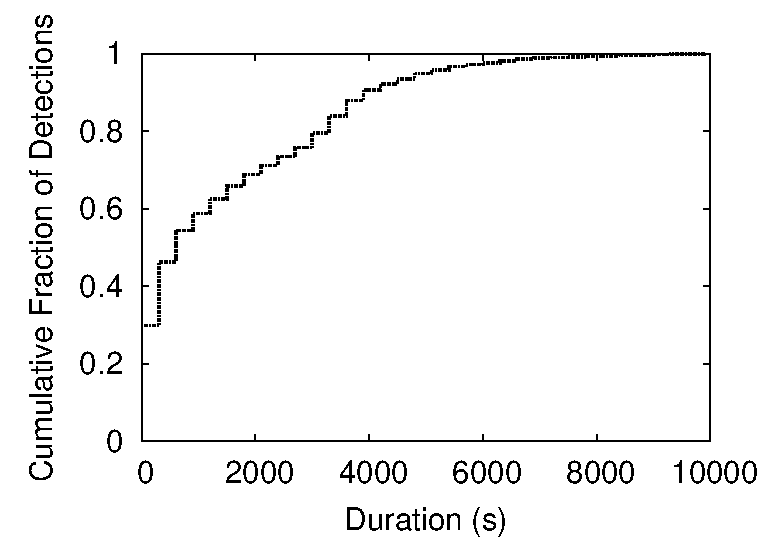
\includegraphics[width=1.05\columnwidth]{figs/patching/durationdetection/durationdetection.eps}
\caption{CDF of detection duration to remap overlappinh routes. }
\label{fig:overlap.delay.cdf}
%
\end{minipage}
\hfill
\begin{minipage}{0.32\textwidth}
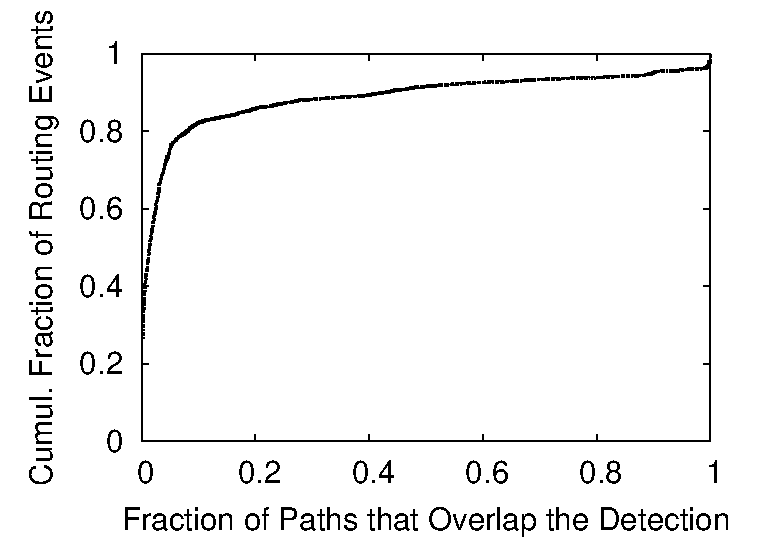
\includegraphics[width=1.05\columnwidth]{figs/patching/routesoverlapping/routesoverlapping.eps}
\caption{CDF of detection overlapping with other routes.}
\label{fig:overlap.quantity.cdf}
\end{minipage}
%
\hfill
\begin{minipage}{0.32\textwidth}
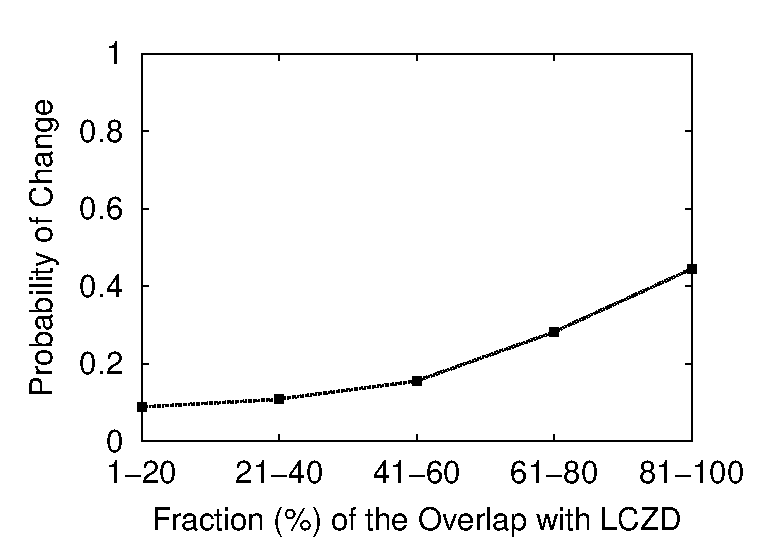
\includegraphics[width=1.05\columnwidth]{figs/patching/probchange/probchange.eps}
\caption{Probability of a overlapping path has a change given the size of the overlap.}
\label{fig:overlap.change.prob}
\end{minipage}
\end{figure*}


Figure~\ref{fig:overlap.delay.cdf} shows the CDF, over all detected
path changes, of the time it takes to remap all
overlapping paths ($|E_p|$) grouped in 5-minute intervals.  
Because we remap overlapping paths within
a short period, there is a lower probability that subsequent routing
events will happen while the remap is ongoing.

Figure~\ref{fig:overlap.quantity.cdf} shows the CDF, over all
detected path changes, of the fraction of paths that overlap with $E_p$.  
We observe that 73.68\% of all routes have at least one 
\emph{overlapping path} which lead us to investigate further if these
paths also change and how the overlapping interval can help us detect the change.
As described in section~\ref{sec:char}, a path can have more than one
$\lczd$. This means that if $E_p$ has more than one $\lczd$, the \emph{overlapping
paths} can cross different parts of $E_p$. Thus, we can divide $E_p$ in a more
fine-grained parts ($\lczd$) which can explain better the behaviour of changes in
\emph{overlapping paths}. For the rest of this section, we
consider each $\lczd$ in $E_p$ independently and we use the notation $E_p[\lczd]$ 
to indicate it. 

Let $O$ denote the overlap between an \emph{overlapping path} $q$ and a 
$E_p[\lczd]$, i.e., $O = E_p[\lczd],\cap\,q$. The next step 
is to analyze whether an \emph{overlapping path} changes given $O$.
Figure~\ref{fig:overlap.change.prob} shows
the fraction of overlapping paths that have changed as well, grouping
\emph{overlapping paths} by the fraction of the \emph{overlapping path}
that overlaps $E_p[\lczd]$, i.e.,
$|O|\div|E_p[\lczd]|$.  We note that as overlapping paths
have more in common with the local change zone domain, the higher
the probability that the overlapping path will change. 

We now want to find a way to identify whether an \emph{overlapping path}
has changed (or remained stable). As pointed out before, a path can have more
than one $\lczd$ and we treat each of them independently in $E_p$.
We now formalize how we consider this fact inside \emph{overlapping paths}.
Let $\lczd'$ denote the local change zone domain of an \emph{overlapping path}
without $r_d$ in all cases and $r_c$ if $|\lczd'_{p}| = |\lczd'_{p-1}|$, i.e.,
$\lczd'$ is the set of hops that reveal changes if probed. We define the
overlapping change set $OCS = \bigcup(\lczd')$ as the set of all hops in the
\emph{overlapping path} that a probe can detect a change.
We also define the Candidates Probing Set ($CPS$) as the subpath 
in the \emph{overlapping path} $q$ between the \textbf{first} and \textbf{last} 
hop in $O$, i.e., a set of hops related to $E_p[\lczd]$ which we want analyze
to determine if $q$ changed. A study on the effectiveness of $r_d$ and $r_c$ 
from $E_p[\lczd]$ in the change detection in \emph{overlapping path}, i.e.,
$r_d \cap OCS$ and $r_c \cap OCS$ reveals that in 99.56\% of times 
$r_d \cap OCS = \emptyset$ and in 91.12\% $r_c \cap OCS = \emptyset$.
For this reason, we exclude the $r_d$ and $r_c$ from $CPS$.

Analyzing all 67 millions overlap found, 66\% of cases crosses overlapping paths 
that does not have any change ($OCS = \emptyset$) and 4,83\% of overlaps have 
$OCS \ne \emptyset$ but $CPS \cap OCS = \emptyset$, 
i.e., we are not able to detect a change in the \emph{overlapping path}
based on the overlap it have with $E_c[\lczd]$. 
We now focus on the 29.07\% of overlaps such that $CPS \cap OCS \ne \emptyset$
where we can make a contribution. Figure~\ref{fig:lczd.intersection}  
shows the distribution of the number of hops in $CPS$ that are in a $OCS$ by the size of $CPS$,
i.e., $|(CPS \cap OCS)| \div |CPS|$.  The distribution shows that,
in 96.70\% of overlaps where $CPS \cap OCS \ne \emptyset$, probing any hop inside $CPS$ 
will detect a change.

%We also looked
%at where the intersection $I$ is located compared to $\lczd$.  We
%find that XX\% of the intersections $I$ are at the start of the
%local change zone (i.e., $r_d + 1$), YY\% of the intersections $I$
%are at the end of the local change zone (i.e., $r_c - 1$), and that
%only ZZ\% of the intersections do are in neither extreme of the
%change zone.


\begin{figure}
\begin{center}
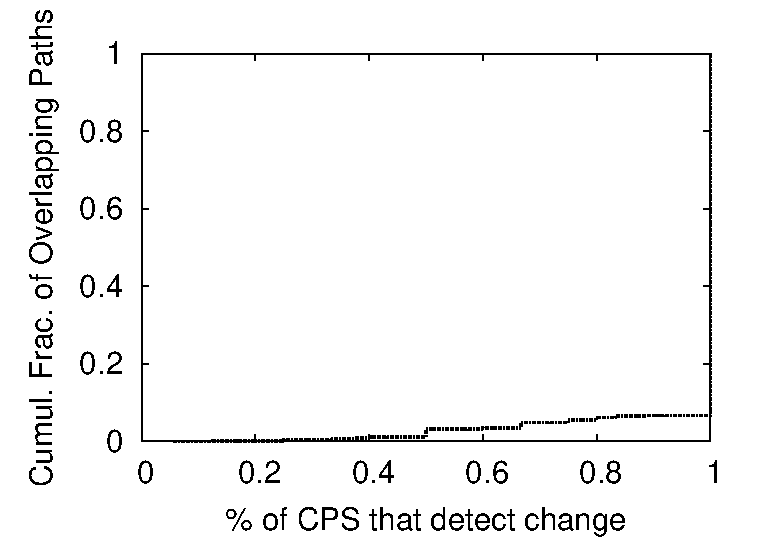
\includegraphics[width=0.8\columnwidth]{figs/patching/overlapcoverage/overlapcoverage_only_lczd.eps}
\caption{Probability of a probe inside a $CPS$ detect a change if $CPS \cap C \ne \emptyset$.}
\label{fig:lczd.intersection}
\end{center}
%
\end{figure}
